\documentclass[%margin%,line,pifont,palatino,courier
]{article}
\usepackage{fullpage}
\usepackage{lastpage}
\usepackage[top=1in,bottom=1in,margin=1in]{geometry}
\usepackage{supertabular}
\usepackage{graphicx,tikz}	
%\usepackage{tkz-euclide}
%\usetkzobj{all}
%\usetikzlibrary{calc}
\usepackage{array,multicol}
\usepackage{amsmath,amssymb}
\usepackage{enumitem}

\usepackage{fancyhdr}
\pagestyle{fancy}

\addtolength{\topmargin}{-0.25in}

\newcommand{\vect}[1]{\mathbf{#1}}
\DeclareMathOperator{\proj}{proj}

\fancypagestyle{plain}{
	\addtolength{\headheight}{0.485in}
	\rhead{\bf MATH 2574 (Calculus III) \\
		%\vspace{0.5pc}
		due Fri 3 Feb 2017 \\}
	\rfoot{\footnotesize $\;$Quiz 1TH, p. \thepage\ (of \pageref{LastPage})
	}
\renewcommand{\headrulewidth}{0pt}
}
\fancyhf{}
\renewcommand{\headrulewidth}{0pt}
\rfoot{\footnotesize Quiz 1TH, p. \thepage\ (of \pageref{LastPage})$\;$}

\title{\vspace{-3.5pc} 
	\flushleft \bf \Large Take-Home Quiz 1: \\ Vectors and vector-valued functions (\S 11.1-11.7)}
\date{}

% % % % %
\begin{document}
\maketitle

\vspace{-3pc}
\noindent{\bf Directions:} This quiz is due on Februrary 3, 2017 at the beginning of lecture.  You may use whatever resources you like -- e.g., other textbooks, websites, collaboration with classmates -- to complete it \textbf{but YOU MUST DOCUMENT YOUR SOURCES}.  Acceptable documentation is enough information for me to find the source myself.  Rote copying another's work is unacceptable, regardless of whether you document it.  

\noindent\hrulefill

\begin{enumerate}
% % %
%\item {\bf 11.1 \#56} Which has a greater horizontal component: a 100-N force directed at an angle of 60 degrees above the horizontal or a 60-N force directed at an angle of 30 degrees above the horizonal? 

% % %
%\item {\bf 11.1 \#66} Let $\vect u=\langle 2,-3\rangle$ and $\vect v=\langle -4,1\rangle$.  Solve the following equation for the vector $\vect x$:
%\[
%-4\vect x=\vect u-8\vect v
%\]

% % %
\item %{\bf 11.1 \#68} 
A sum of scalar multiples of two or more vectors (such as $c_1\vect u+c_2\vect v+c_3\vect w$, where $c_i$ are scalars) is called a \textbf{linear combination} of the vectors.  Express $\langle 4,-8\rangle$ as a linear combination of the vectors $\vect u=\langle 1,1\rangle$ and $\vect v=\langle -1,1\rangle$. 

% % %
%\item {\bf 11.1 \#70} Solve the following system of equations for the vectors $\vect u$ and $\vect v$:
%\begin{align*}
%2\vect u+3\vect v &= \vect e_1 \\
%\vect u-\vect v &= \vect e_2
%\end{align*}

% % %
%\item {\bf 11.1 \#72} Find the vector that is 3 times $\langle 3,-5\rangle$ plus -9 times $\langle 6,0\rangle$.

% % %
%\item {\bf 11.1 \#76} An ant walks due east at a constant speed of 2 mi/hr on a sheet of paper that rests on a table.  Suddenly, the sheet of paper starts moving southeast at $\sqrt2$ mi/hr.  Describe the motion of the ant relative to the table.

% % %
%\item {\bf 11.2 \#26} Find an equation or inequality that describes a ball with center $(0,-2,6)$ witht he point $(1,4,8)$ on its boundary.

% % %
%\item {\bf 11.2 \#28} Find an equation of the sphere passing through the point $P=(-4,2,3)$ and $Q=(0,2,7)$ with its center at the midpoint of $PQ$.

% % %
\item %{\bf 11.2 \#36} 
Give a geometric description of the following set of points:
\[
x^2+y^2+z^2-8x+14y-18z\geq 65
\]

% % %
%\item {\bf 11.2 \#38} Give a geometric description of the following set of points:
%\[
%x^2-4x+y^2+6y+z^2+14=0
%\]

% % %
%\item {\bf 11.2 \#56} An object is acted upon by the forces $\vect F_1=\langle 10,6,3\rangle$ and $\vect F_2=\langle 0,4,9\rangle$.  Find the force $\vect F_3$ that must act on the object so that the sum on the forces is zero.

% % %
\item %{\bf 11.2 \#64} 
Give a geometric description of the set of points $(x,y,z)$ that lie on the intersection of the sphere $x^2+y^2+z^2=36$ and the plane $z=6$.

% % %
%\item {\bf 11.2 \#70} Find a vector of length 3 that is parallel to $\vect v=\vec{PQ}$, with $P=(1,0,1)$ and $Q=(2,-1,1)$.

% % %
%\item {\bf 11.2 \#72} Determine the values of $x$ and $y$ such that the points $(1,2,3)$, $(4,7,1)$, and $(x,y,2)$ are collinear.

% % %
%\item {\bf 11.2 \#74} An object on an inclined plane does not slide provided the component of the object's weight parallel to the plane $|\vect W_{\text{par}}|$ is less than or equal to the magnitude of the opposing frictional force $|\vect F_{\text f}|$.  The magnitude of the frictional force, in turn, is proportional to the component of the object's weight perpendicular to the plane $|\vect W_{\text{par}}|$ (accompanying picture).  The constant of proportionality is the coefficient of static friction $\mu>0$.
%\begin{enumerate}
%	\item Suppose a 100-lb block rests on a plane that is tilted at an angle of $\theta=20^{\circ}$ to the horizontal.  Find $|\vect W_{\text{par}}|$ and $|\vect W_{\text{perp}}|$.
%	\item The condition for the block not sliding is $|\vect W_{\text{par}}|\leq \mu |\vect W_{\text{perp}}|$.  If $\mu=0.65$, does the block slide?
%	\item What is the critical angle above which the block slides with $\mu=0.65$? 
%\end{enumerate}

% % %
%\item {\bf 11.2 \#80} For constants $a,b,c,$ and $d,$ show that the equation
%\[
%x^2+y^2+z^2-2ax-2by-2cz=d
%\]
%describes a sphere centered at $(a,b,c)$ with radius $r$, where $r^2=d+a^2+b^2+c^2>0$.

% % %
%\item {\bf 11.3 \#28}

% % %
%\item {\bf 11.3 \#38} A stroller is pushed 20 m with a constant force of 10 N at an angle of 15 degrees below the horizontal.  Calculate the work done.

% % %
%\item {\bf 11.3 \#40} A constant force $\vect F=\langle 4,3,2\rangle$ (in newtons) moves an object from $(0,0,0)$ to $(8,6,0)$.  Calculate the work done.

% % %
%\item {\bf 11.3 \#46} Find the components of the vertical force $\vect F=\langle 0,-10\rangle$ in the directions parallel and normal (perpendicular) to the plane that makes an angle of $\theta=\arctan{\frac{4}{3}}$ with the positive $x$-axis.

% % %
%\item {\bf 11.3 \#50} Describe all unit vectors orthogonal to $\vect v=\vect e_1+\vect e_2+\vect e_3$.

% % %
%\item {\bf 11.3 \#52} Find two vectors that are orthogonal to $\langle 0,1,1\rangle$ and to each other.

% % %
%\item {\bf 11.3 \#60} Let $\vect u=\langle 4,3,0\rangle$ and $\vect v=\langle 1,1,1\rangle$.  Express $\vect u$ as the sum $\vect u=\vect p+\vect n$, where $\vect p$ is parallel to $\vect v$, and $\vect n$ is normal to $\vect v$.

% % %
\item %{\bf 11.3 \#64} 
Carry out the following steps to determine the (least) distance between the point $P=(0,2,6)$ and the line $\ell$ that is parallel to the $\langle 3,0,-4\rangle$ and passes through the origin.
\begin{enumerate}
	\item Find any vector $\vect v$ in the direction of $\ell$.
	\item Find the position vector corresponding to $P$.
	\item Find $\proj_{\vect v}\vect u$.
	\item Show that $\vect w=\vect u-\proj_{\vect v}\vect u$ is a vector orthogonal to $\vect v$ whose length is the distance between $P$ and the line $\ell$.
	\item Find $\vect w$ and $|\vect w|$.  Why is $|\vect w|$ the least distance between $P$ and $\ell$?
\end{enumerate}

% % %
%\item {\bf 11.3 \#68} Write the vector $\langle 2,-6\rangle$ in terms of $\vect I=\langle \frac{1}{\sqrt 2},\frac{1}{\sqrt 2}\rangle$ and $\vect J=\langle -\frac{1}{\sqrt 2},\frac{1}{\sqrt 2}\rangle$.

% % %
%\item {\bf 11.3 \#72} Suppose water flows in a thin sheet over the $xy$-plane with a uniform velocity given by the vector $\vect v=\langle 1,2\rangle$; this means that at all points of the plane, the velocity of the water has components 1 m/s in the $x$-direction and 2 m/s in the $y$-direction (see figure).  Let $C$ be an imaginary unit circle (that does not interfere with the flow).
%\begin{enumerate}
%	\item Show that at the point $(x,y)$ on the circle $C$, the outward-pointing vector normal to $C$ is $\vect n=\langle x,y\rangle$.
%	\item Show that at the point $(\cos{\theta},\sin{\theta})$ on the circle $C$, the outward-pointing vector normal to $C$ is also $\vect n=\langle \cos{\theta},\sin{\theta}\rangle$.
%	\item Find all points on $C$ at which the velocity is normal to $C$.
%	\item Find all points on $C$ at which the velocity is tangential to $C$.
%	\item At each point on $C$, find the component of $\vect v$ normal to $C$. Express the answer as a function of $(x,y)$ and as a function of $\theta$.
%	\item What is the net flow through the circle?  That is, does water accumulate inside the circle?
%\end{enumerate}

% % %
%\item {\bf 11.3 \#74} The German mathematicialn Gauss proved that the densest wayto pack circles with the same radius in the plane is to place the centers of the circles on a hexagonal grid (see figure).  Some molecular stuctures use this packing or its three-dimensional analog.  Assume all circles have a radius of 1 and let $\vect r_{ij}$ be the vector that extends from the center of the circle $i$ to the center of the circle $j$, for $i,j=0,1,\dots, 6$.
%\begin{enumerate}
%	\item Find $\vect r_{0j}$, for $j=1,2,\dots, 6$.
%	\item Find $\vect r_{12}$, $\vect r_{34}$, and $\vect r_{61}$.
%	\item Imagine circle 7 is added to the arrangement as shown in the figure.  Find $\vect r_{07}$, $\vect r_{17}$, $\vect r_{47}$, and $\vect r_{75}$.
%\end{enumerate}

% % %
%\item {\bf 11.3 \#82} Recall that two lines $y=mx+b$ and $y=nx+c$ are orthogonal provided $mn=-1$ (the slopes are negative reciprocals of each other).  Prove that the condition $mn=-1$ is equivalent to the orthogonality condition $\vect u\cdot \vect v=0$, where $\vect u$ points in the direction of one line and $\vect v$ points in the direction of the other line.

% % %
%\item {\bf 11.3 \#90} Use projections to find a general formula for the (least) distance between the oint $P=(x_0,y_0)$ and the line $ax+by=c$.  (See Exercises 62-65).

% % %
%\item {\bf 11.4 \#24} Find the area of the parallelogram that has two adjacent sides $\vect u=8\vect i+2\vect j-3\vect k$ and $\vect v=2\vect i+4\vect j-4\vect k$.

% % %
%\item {\bf 11.4 \#38} Find a vector orthogonal to $\langle 6,-2,4\rangle$ and $\langle 1,2,3\rangle$.

% % %
\item %{\bf 11.4 \#46} 
A particle with a unit negative charge ($q=-1$) enters a constant magnetic field $\vect B=5\vect k$ with a velocity $\vect v=\vect i+2\vect j$.  Find the magnitude and direction of the force on the particle.  Make a sketch of the magnetic field, the velocity, and the force.

% % %
%\item {\bf 11.4 \#48} A proton ($q=1.6\times 10^{-19}$ C) with velocity $2\times 10^6 \vect j$ m/s experiences a force in newtons of $\vect F=5\times 10^{-12}\vect k$ as it passes through the origin.  Find the magnitude and direction of the magnetic field at that instant.

% % %
%\item {\bf 11.4 \#52} Find the value of $a$ such that 
%\[
%\langle a,a,2\rangle \times \langle 1,a,3\rangle =\langle 2,-4,2\rangle.
%\]

% % %
\item %{\bf 11.4 \#56} 
Find the area of the triangle with vertices $O=(0,0,0)$, $P=(2,4,6)$, and $Q=(6,5,4)$.

% % %
%\item {\bf 11.4 \#60} Find all vectors $\vect u$ that satisfy the equation
%\[
%\langle 1,1,1\rangle \times \vect u = \langle 0,0,1\rangle.
%\]

% % %
%\item {\bf 11.4 \#62} Express $\vect u$, $\vect v$, and $\vect w$ in terms of their components and then show that $\vect u\cdot (\vect v\times \vect w)$ equals the determinant
%\[
%\begin{vmatrix}
%u_1 & u_2 & u_3 \\
%v_1 & v_2 & v_3 \\
%w_1 & w_2 & w_3
%\end{vmatrix}.
%\]

% % %
%\item {\bf 11.4 \#66} A horizontally outstrectched arm supports a weight of 20 lb in a hand (see figure).  If the distance from the shoulder to the elbow is 1 ft and the distance from the elbow to the hand is 1 ft.  Find the magnitude and describe the direction of the torque about 
%\begin{enumerate}
%	\item the shoulder and 
%	\item the elbow (the units of torque in this case are ft-lb).
%\end{enumerate}

% % %
%\item {\bf 11.5 \#22} Find an equation for the line through $(0,2,1)$ that is perpendicular to both $\vect \langle 4,3,-5\rangle$ and the $z$-axis.

% % %
%\item {\bf 11.5 \#24} Find an equation for the line through $(1,0,-1)$ that is perpendicular to the lines $\vect r_1=\langle 3+2t,3t,-4t\rangle$ and $\vect r_2=\langle t,t,-t\rangle$.

% % %
%\item {\bf 11.5 \#34} Graph the following curve and indicate its orientation:
%\[
%\vect r(t)=4\sin t\vect i+4\cos t\vect j +e^{-t/10}\vect k\text{, for }0\leq t<\infty.
%\]

% % %
%\item {\bf 11.5 \#36} Graph the following curve and indicate its orientation:
%\[
%\vect r(t)=e^{-t/10}\vect i+3\cos t\vect j+3\sin t\vect k\text{, for } 0\leq t<\infty.
%\]

% % %
%\item {\bf 11.5 \#38} Graph the following curve and indicate its orientation:
%\[
%\vect r(t)=2\cos t\vect i+4\sin t\vect j+\cos{10t}\vect k\text{, for } 0\leq t\leq 2\pi.
%\]

% % %
%\item {\bf 11.5 \#40} Graph the following curve and indicate its orientation:
%\[
%\vect r(t)=\cos t\sin{3t}\vect i+\sin t\sin{3t}\vect j+\sqrt t\vect k\text{, for } 0\leq t\leq 9.
%\]

% % %
%\item {\bf 11.5 \#48} Determine an equation of the line that is perpendicular to the lines $\vect r(t)=\langle -2+3t,2t,3t\rangle$ and $\vect R(s)=\langle -6+s,-8+2s,-12+3s\rangle$ and passes through the point of intersection of the lines $\vect r$ and $\vect R$.

% % %
\item %{\bf 11.5 \#68} 
Consider the lines
\begin{align*}
\vect r(t) &= \langle 2+2t,8+t,10+3t\rangle \text{ and } \\
\vect R(s) &= \langle 6+s,10-2s,16-s\rangle.
\end{align*}
\begin{enumerate}
\item Determine whether the lines intersect (have a common point) and if so, find the coordinates of the point.
\item If $\vect r$ and $\vect R$ describe the paths of the two particles, do the particles collide?  Assume that $t\geq 0$ and $s\geq 0$ measure time in seconds, and that motion starts at $s=t=0$.
\end{enumerate}

% % %
%\item {\bf 11.5 \#70} Consider the curve 
%\[
%\vect r(t)=(a\cos t+b\sin t)\vect i +(c\cos t+d\sin t)\vect j+(e\cos t+f\sin t)\vect k\text{, where $a,b,c,d,e,f$ are real numbers. }
%\]
%This curve lies in a plane; show that it is a circel centered at the origin with radius $R$ provided 
%\[
%a^2+c^2+e^2=b^2+d^2+f^2=R^2\text{ and } ab+cd+ef=0.
%\]

% % %
%\item {\bf 11.5 \#74} A golfer launches a tee shot down a horizontal fairway; it follows a path given by $\vect r(t)=\langle at,(75-0.1a)t,-5t^2+80t\rangle$, where $t\geq 0$ measures time in seconds and $\vect r$ has units of feet.  The $y$-axis points straight down the fairway and the $z$-axis points vertically upward.  The parameter $a$ is the slice factor that determines how much the shot deviates from a straight path down the fairway.
%\begin{enumerate}
%	\item With no slice ($a=0$), sketch and describe the shot.  How far does the ballt ravel horizontally (the distance between the ponit the ball leaves the ground and the point where it first strikes the ground)?
%	\item With a slice $(a=0.2$), sketch and describe the shot.  How far does the ball travel horizontally?
%	\item How far does the ball travel horizontally with $a=2.5$?
%\end{enumerate}

% % %
%\item {\bf 11.5 \#76} Prove that for integers $m$ and $n$, the curve
%\[
%\vect r(t)=\langle a\sin(mt)\cos(nt),b\sin(mt)\sin(nt),c\cos(mt)\rangle
%\]
%lies on the surface of a sphere provided $a^2+b^2=c^2$.

% % %
%\item {\bf 11.6 \#24} Find the unit tangent vector for 
%\[
%\vect r(t)=\langle \sin t,\cos t,\cos t\rangle\text{, for }0\leq t\leq 2\pi.
%\]

% % %
\item %{\bf 11.6 \#28} 
Find the unit tangent vector at $t=0$ for 
\[
\vect r(t)=\langle \sin t,\cos t,e^{-t}\rangle\text{, for }0\leq t\leq \pi.
\]

% % %
%\item {\bf 11.6 \#32} Let $\vect v(t)=e^t\vect i+2e^{-t}\vect j-e^{2t}\vect k$.  Compute the derivative of $(4t^8-6t^3)\vect v(t)$.

% % %
%\item {\bf 11.6 \#46} Compute $\vect r'(t)$ and $\vect r''(t)$ for 
%\[
%\vect r(t)=\tan t\vect i+\left(t+\frac{1}{t}\right)\vect j-\ln(t+1)\vect k.
%\]

% % %
%\item {\bf 11.6 \#58} Find the function $\vect r$ that satisfies 
%\begin{align*}
%\vect r'(t) &= \frac{t}{t^2+1}\vect i+te^{-t^2}\vect j-\frac{2t}{\sqrt{t^2+4}}\vect k \\
%\vect r(0) &= \vect i +\frac{3}{2}\vect j-3\vect k
%\end{align*}

% % %
%\item {\bf 11.6 \#66} Evaluate
%\[
%\int_0^{\pi/4}(\sec^2t\vect i-2\cos t\vect j-\vect k)\ dt.
%\]

% % %
%\item {\bf 11.6 \#70} Find an equation for the line tangent to 
%\[
%\vect r(t)=\langle \sqrt{2t+1},\sin{\pi t},4\rangle
%\]
%at $t=4$.  Choose an orientation for the line that is the same as the direction of $\vect r'$.

% % %
%\item {\bf 11.6 \#72} Let $\vect u(t)=\langle 1,t,t^2\rangle$.  Compute the derivative of $\vect u(t^3)$.

% % %
\item %{\bf 11.6 \#80} 
Consider the curve 
\[
\vect r(t)=\langle \sqrt t,1,t\rangle,
\]
for $t>0$.  Find all points on the curve at which $\vect r$ and $\vect r'$ are orthogonal.

% % %
%\item {\bf 11.6 \#90} 
%Prove that $\vect r$ describes a curve that lies on the surface of a sphere centered at the origin ($x^2+y^2+z^2=a^2$ with $a\geq 0$) if and only if $\vect r$ and $\vect r'$ are orthogonal at all points of the curve.

% % %
%\item {\bf 11.7 \#68} Consider an object moving on a cycloid with the position function $\vect r(t)=\langle t-\sin t,1-\cos t\rangle$, for $0\leq t\leq 4\pi$.
%\begin{enumerate}
%	\item Graph the trajectory.
%	\item Find the velocity and speed of the object.  At what point(s) on the trajectory does the object move fastest?  Slowest?
%	\item Find the acceleration of the object and show tat $|\vect a(t)|$ is constant.
%	\item Explain why the trajectory has a cusyp at $t=2\pi$.
%\end{enumerate}

% % %
%\item {\bf 11.7 \#70} A golfer stands 390 ft (130 yd) horizontally from the hole and 40 ft below the hole (see figure).  Assuming the ball is hit with an initial speed of 150 ft/s, at what angle(s) should it be ht to land in the hole?  Assume that the path of the ball lies in a plane.

% % %
%\item {\bf 11.7 \#72} A golfer stands 390 ft horizontally from the hole and 40 ft below the hole (see figure).  If the ball leaves the ground at an initial angle of $45^{\circ}$ with the horizontal, with what initial velocity should it be hit to land in the hole? 

% % %
\item %{\bf 11.7 \#74} 
The lip of a ski jump is 8 m above the outrun that is sloped at an angle of 30 degrees to the horizontal (see figure).

\centering{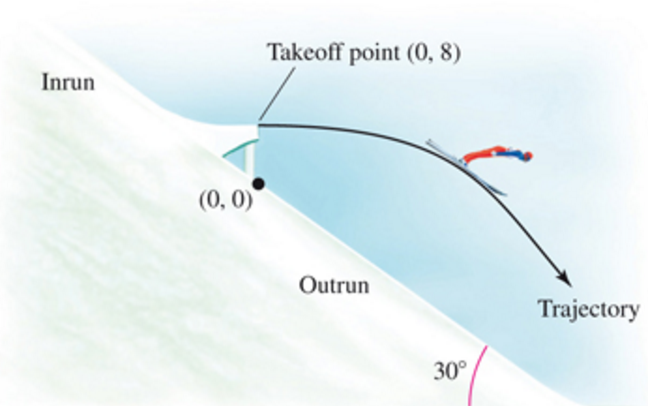
\includegraphics[scale=0.75]{Q1SkiProb}
}
\begin{enumerate}
	\item If the initial velocity of a ski jumper at the lip of the jump is $\langle 40,0\rangle$ m/s, what is the length of the jump (distance from the origin to the landing point)?  Assume only gravity affects the motion.
	\item Assume that air resistance produces a constant horizontal acceleration of 0.15 m/s$^2$ opposing the motion.  What is the length of the jump?
	\item Suppose that the takeoff ramp is titlted upward at an angle of $\theta$, so that the skier's initial velociy is $40\langle \cos{\theta},\sin{\theta}\rangle$ m/s.  What value of $\theta$ maximizes the length of the jump?  Express your answer in degrees and neglect air resistance.
\end{enumerate}

% % %
%\item {\bf 11.7 \#76} Assume an object is launched from the origin with an initial speed $|\vect v_0|$ at an angle $\alpha$ to the horizontal, where $0<\alpha<\frac{\pi}{2}$.
%\begin{enumerate}
%	\item Find the time of flight, range, and maximum height (relative to the launch point) of the trajectory if the ground slopes downward at a constant angle $\theta$ from the launch site, where $0<\theta<\frac{\pi}{2}$.
%	\item Find the time of flight, range, and maximum heght of the trajectory if the ground slopes upward at a constant angle of $\theta$ from the launch site.  Assume $\tan{\theta}<\frac{1}{2}\tan{\alpha}$.
%\end{enumerate}

% % %
%\item {\bf 11.7 \#80} Consider the ellipse $\vect r(t)=a\cos t,b\sin t\rangle$, for $0\leq t\leq 2\pi$, where $a$ and $b$ are real numbers.  Let $\theta$ be the angle between the position vector and the $x$-axis.
%\begin{enumerate}
%	\item Show that $\tan{\theta}=(b/a)\tan t$.
%	\item Find $\theta'(t)$.
%	\item The area bounded by a polar curve $f(\theta)$ on the interval $[0,\theta]$ is 
%	\[
%	A(\theta)=\frac{1}{2}\int_0^{\theta}(f(u))^2\ du.
%	\]
%	Letting $f(\theta(t))=|\vect r(\theta(t))|$, show that $A'(t)=\frac{1}{2}ab$.
%\end{enumerate}



% % % % %
\end{enumerate}
\end{document}